\documentclass[dvipdfmx]{article}
\usepackage[dvipdfmx]{graphicx}
\usepackage{amsmath, amssymb}
\usepackage{mathtools}
\usepackage{here}
\usepackage{url}

\begin{document}
\title{Weekly Report}
\author{Riku Gondow}
\maketitle
\section{Progress}
\begin{itemize}
    \item Implement open-set identification on the 30-subjects dataset\cite{dataset} as a baseline method.
\end{itemize}

\section{Implementation detail}

\begin{figure}[H]
    \begin{center}
    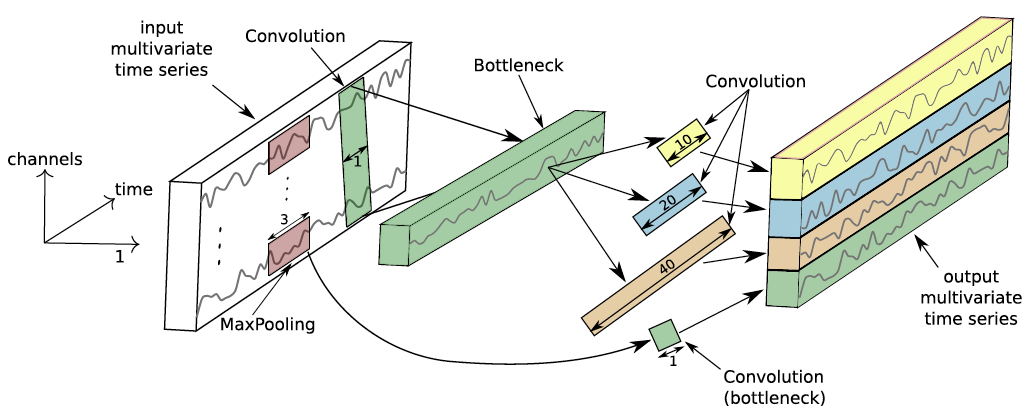
\includegraphics[width=0.8\linewidth]{./img/Incep.png}
    \end{center}
    \caption{The architecture of InceptionTime}
\end{figure}
    
Using a model called Inception Time\cite{Inception}, we tried identifying 30-subjects using heartbeat signals generated from radar. Table1 shows the hyper parameter, and Adam was used as an optimizer.


\begin{table}[H]
    \caption{Hyper parameter}
    \centering
    \begin{tabular}{cc}
    \hline
    batch size & 64 \\
    learning rate & 0.001 \\
    epochs & 10 \\
    Sampling rate & 250 Hz \\
    window size & 5s \\
    overlap & 1.5s \\
    \hline
    \end{tabular}
\end{table}

Here is the definition of the openness index\cite{Heart signature}. 

\begin{equation}\label{}
openness = 1 - \sqrt{\frac{C_{train}}{C_{test}}}
\end{equation}

where $C_{train}$ and $C_{test}$ are the number of known identities in the training
and test set, respectively. The openness index is used to quantify how
many unknowns a model encounter during testing. The higher the index
is, the more difficult the problem is.

\section{Results}
A threshold is needed because the Softmax function only outputs labels for the number of classes used in the training. Figure 2 shows the change in accuracy as the threshold value is varied.

\begin{figure}[H]
\begin{center}
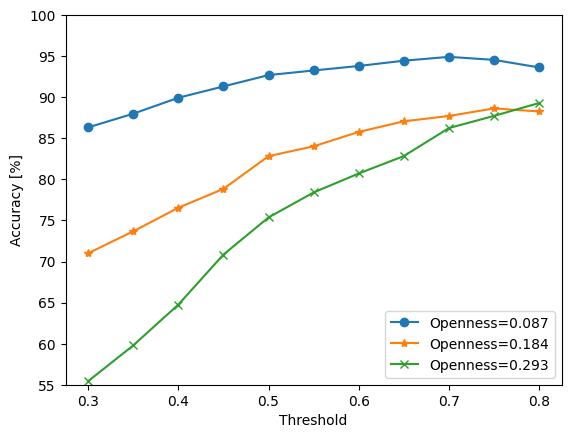
\includegraphics[width=\linewidth]{./img/openset_graph.png}
\end{center}
\caption{Change in Accuracy with Threshold Varying}
\end{figure}

Here is the openness index table. This table shows the correspondence between openness and known/unknown classes.

\begin{table}[H]
    \caption{Correspondence between openness and known/unknown classes}
    \centering
    \begin{tabular}{|c||c|c|}
    \hline
    openness & $C_{train}$/$C_{test}$ & num of unknown \\ \hline
    0.087 & 25/30 & 5 \\ \hline
    0.184 & 20/30 & 10 \\ \hline
    0.293 & 15/30 & 15 \\ \hline
    \end{tabular}
\end{table}

Here is an example of Confusion Matrix. When the threshold is increased, the percentage of correct answers for Unknown labels increases, but the percentage of correct answers for Known labels decreases.

\begin{figure}[H]
    \begin{center}
    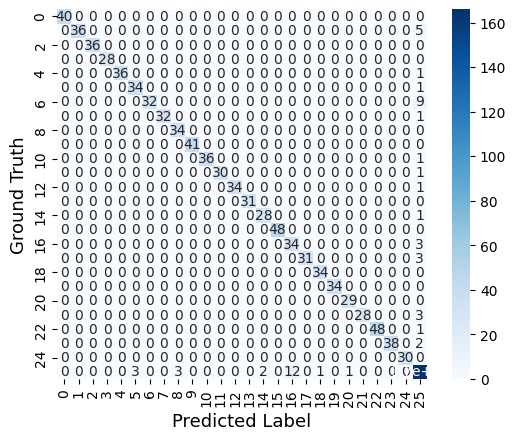
\includegraphics[width=\linewidth]{./img/conf_threshold.png}
    \end{center}
    \caption{Confusion Matrix (openness=0.087, threshold=0.70)}
\end{figure}



\section{Next Plan}
\begin{itemize}
    \item Submit a brief report for graduation thesis to Canvas LMS
    \item Consider improvement plan
    \begin{itemize}
        \item Change the structure of model, loss function
        \item Change the scenario
        \item Evaluate another noisy dataset
    \end{itemize}
\end{itemize}

\begin{thebibliography}{99}
\bibitem{Inception} Ismail Fawaz, H., Lucas, B., Forestier, G. et al. InceptionTime: Finding AlexNet for time series classification. Data Min Knowl Disc 34, 1936–1962 (2020). https://doi.org/10.1007/s10618-020-00710-y
\bibitem{dataset} \url{https://figshare.com/articles/dataset/A_dataset_of_clinically_recorded_radar_vital_signs_with_synchronised_reference_sensor_signals/12186516?file=22515782}
\bibitem{Heart signature} Yan, Baiju, et al. ”Heart signatures: Open-set person identification based on cardiac radar signals.” Biomedical Signal Processing and Control 72 (2022): 103306.
\end{thebibliography}
\end{document}